\documentclass[tikz,border=5pt]{standalone}
\usetikzlibrary{spath3,arrows.meta}
\begin{document}
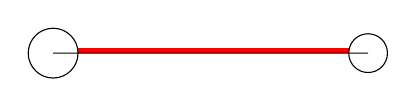
\begin{tikzpicture}
    \path[spath/save=apath] 
    (0,0) foreach \k in {1,...,4} { -- ++(1,0) +(0,0)}; 
    \draw[
        ultra thick,red,
        spath/.cd,
        shorten at end={apath}{7pt}, 
        shorten at start={apath}{9pt}, 
        translate={apath}{0pt}{1pt},%平移1pt
        use=apath,
    ];
    \draw (0,0) 
    circle[radius=9pt] 
    [spath/use=apath] 
    circle[radius=7pt]; 
\end{tikzpicture}

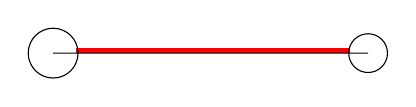
\begin{tikzpicture}
    \path[spath/save=apath] 
    (0,0) foreach \k in {1,...,4} { to[out=0,in=180] ++(1,0) +(0,0)}; 
    \draw[
        ultra thick,red,
        spath/.cd,
        shorten at end={apath}{7pt}, 
        shorten at start={apath}{9pt}, 
        translate={apath}{0pt}{1pt},%平移1pt
        use=apath,
    ];
    \draw (0,0) circle[radius=9pt] [spath/use=apath] circle[radius=7pt]; 
\end{tikzpicture}

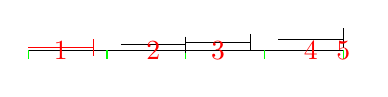
\begin{tikzpicture}
    \draw[spath/save=npath] 
    (0,0) foreach \k in {1,...,4} { -- ++(1,0) +(0,0)};
    \draw[green] 
    (0,0) -- +(0,-3pt) foreach \k in {1,...,4} { --  +(0,-3pt) ++(1,0)} -- +(0,-3pt);

    \tikzset{ 
        spath/.cd,
        insert gaps after components={npath}{10pt}{1,3}, 
        get components of={npath}\components,
    }

    \tikzset{path 1/.style={red}}

    \foreach[count=\k] \cpt in \components {
        \path[ 
            draw,
            path \k/.try,
            spath/.cd, 
            translate=\cpt{0pt}{\k pt}, 
            use=\cpt,
        ] +(0,3pt) -- +(0,-3pt);
        \node[text=red] at (spath cs:{\cpt} .5) {\(\k\)};
    }
\end{tikzpicture}

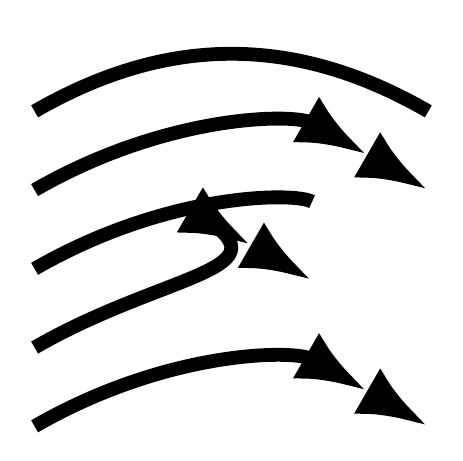
\begin{tikzpicture}[>=Latex, line width=5pt]
    % Just a simple line
    \draw (0,1) to[bend left] +(5,0);
    % Same line but with arrows, also save the path
    \draw[->.>,spath/save=arrow] (0,0) to[bend left] +(5,0);
    % Let’s redraw that path without the arrows - it’s short! But also distorted 
    \draw[spath/use={arrow,transform={yshift=-1cm}}];
    % So if we redraw it with arrows it gets doubly shortened 
    \draw[->.>,spath/use={arrow,transform={yshift=-2cm}}];
    % % If we disable the shortening, the arrows end up in the right place 
    \draw[->.>,spath/use={arrow,transform={yshift=-3cm}},spath/arrow
    shortening=false]; 
\end{tikzpicture}

\end{document}